%%
%% Template chap2.tex
%%

\chapter{Implementing Fingerprint Indexing}
\label{cha:method}

\section{Structure of \Beagle}
\label{sec:initial}

Making any extension to the \beagle\ project (or any sizeable project
for that matter) will obviously require a solid
understanding of the existing codebase. This section provides an overview
of any existing Scala classes and their structure which is relevant to the implementation of the Fingerprint Index.

\subsection{Syntax and Data Structures}

\begin{figure}[h]
  \centering
  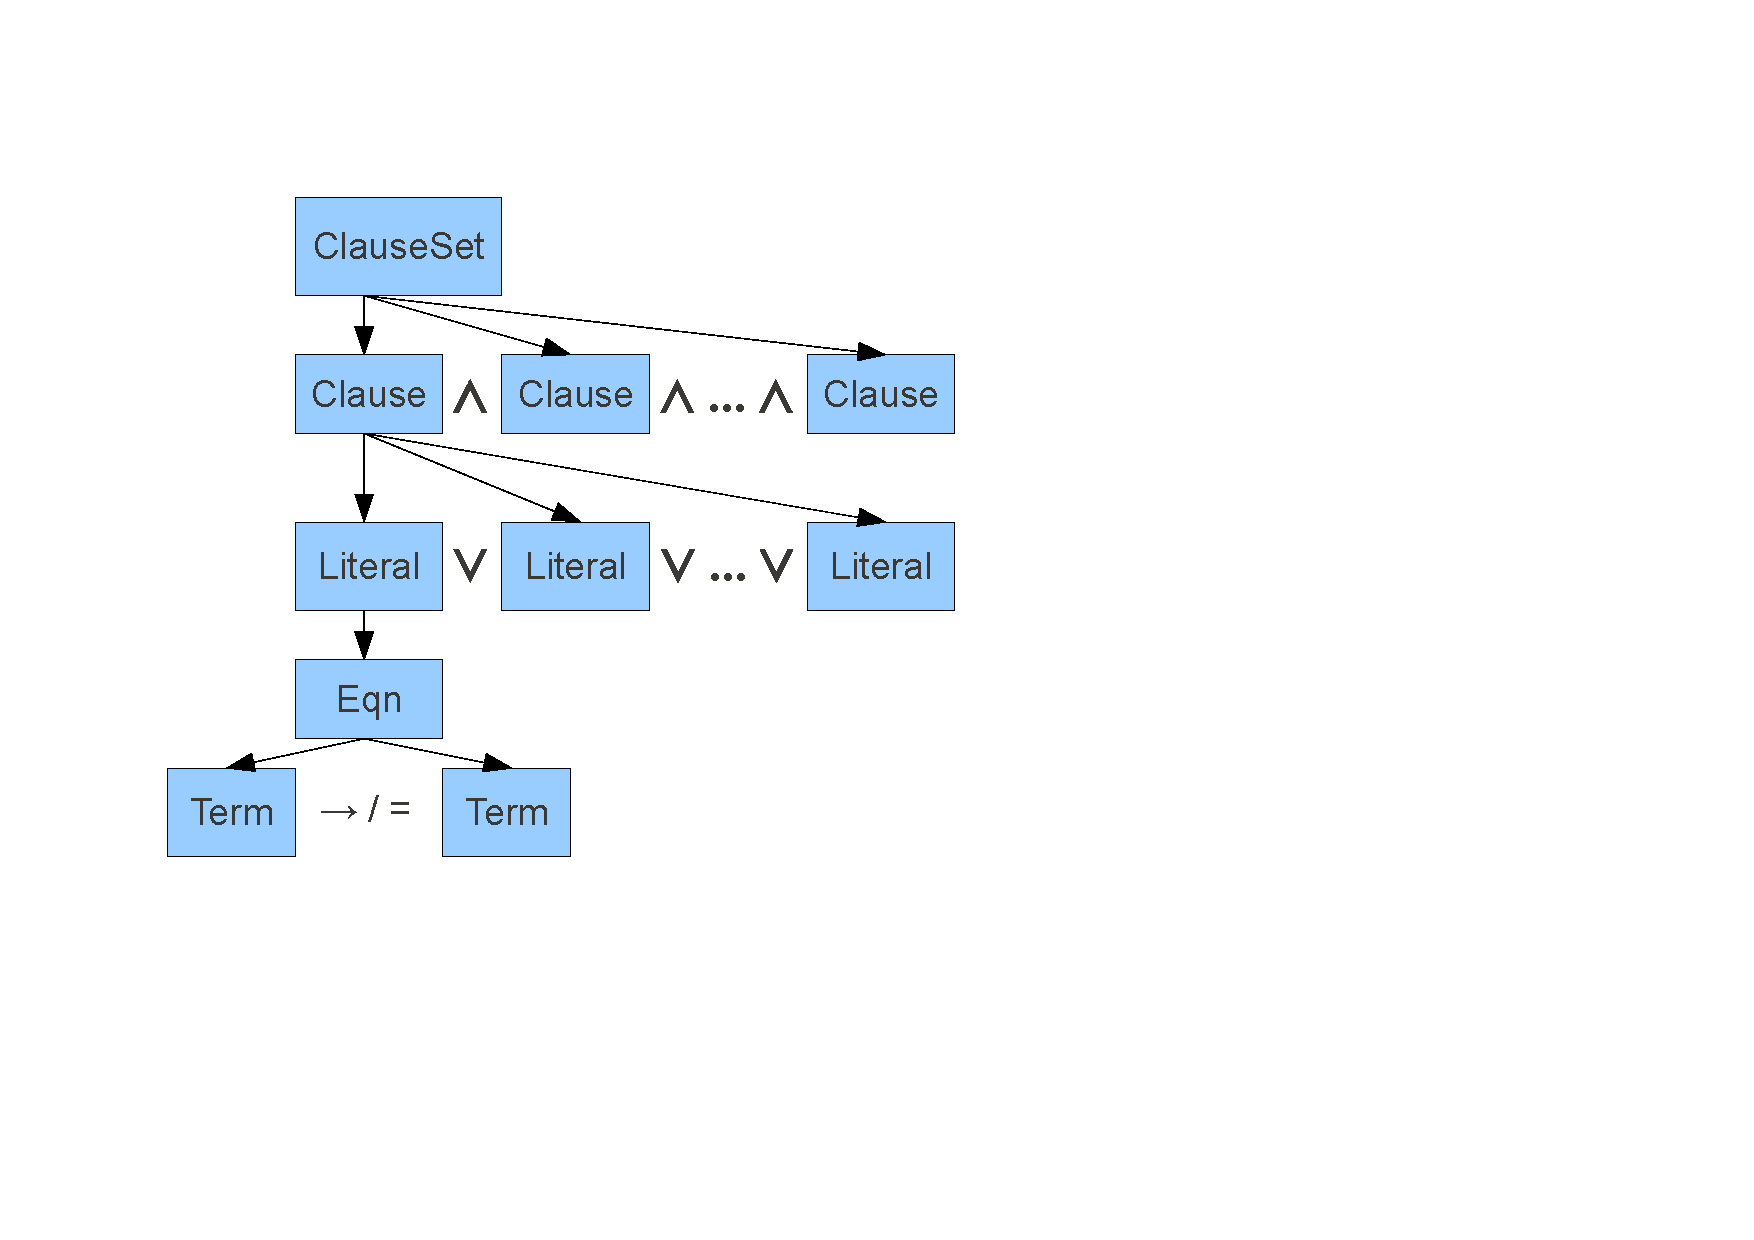
\includegraphics[clip,trim=2.5cm 5cm 10cm 2cm,width=\textwidth]{resources/logicstructure}
  \caption
   {Class structure for internal representation of logical formulae.}
   \label{fig:expressions}
\end{figure}

\subsection{Main Inference Procedure}


\begin{listing}[H]
\begin{lstlisting}
Create two ClauseSets, new and old
While new is not empty
   Select a clause from new, removing it
   Simplify it |\textbf{with respect to all other clauses (new and old)}|
   If the simplified clause is a tautology:
       Continue
   If the simplified clause is the empty clause:
       return UNSAT
   If one of the Define, Split or Inst rules apply:
       Apply the rule
       Add result to new
       Continue
   Add simplified clause to old
   Attempt all inference rules:
       Equality Resolution
       Equality Factoring
       Superposition |\textbf{with respect to all clauses in old}|
   Add all results to new
end While
\end{lstlisting}
\caption{Pseudocode for \beagle's main inference procedure.}
\label{lst:featuredata}
\end{listing}


\section{Building the Fingerprint Indexer}
\label{sec:initial}

The first step in adding Fingerprint Indexing to \beagle\ is creating the indexer
itself; a Scala class which will manage the index and provide functions for adding
to it and retrieving from it. 

\subsection{Objects and Datatypes}

\subsubsection{Fingerprint Features}

\begin{listing}[H]
\begin{scalacode}
/** Pseudo enumerated type for fingerprint features */
sealed abstract class FPFeature
case object FPA extends FPFeature 
case object FPB extends FPFeature
case object FPN extends FPFeature
case class  FPF(val subterm : FunTerm) extends FPFeature
\end{scalacode}
\caption{Data type for the 4 Fingerprint Features \protect\cite[p5]{shulz12}}
\label{lst:featuredata}
\end{listing}

\subsubsection{Positions}

We implement positions in the simple/na\"{\i}ve manner, simply as a list of
Integers (where Nil is used to index the top-level term).

\subsubsection{Term Fingerprints}

\subsubsection{Fingerprint Index}

The final data structure we require is the 

\begin{listing}[H]
\begin{scalacode}
/** Algebraic Data type for our index. Either we are at a leaf
  * (set of terms) or must continue traversal via the map. */ 
sealed abstract class Index
case class Leaf(set: Set[Term])                 extends Index
case class Node(map: HashMap[FPFeature, Index]) extends Index
\end{scalacode}
\caption{Data type for the actual term index. \protect\cite[p7]{shulz12}}
\label{lst:indexdata}
\end{listing}

Note that this Index object does not necessarily take up a significant portion of memory.
All Terms are already stored within the ClauseSet object (See Figure \ref{fig:expressions});
so the Index itself will generally only add a fairly lightweight structure of pointers.


\subsection{Building Term Fingerprints}

The following block of Scala code extracts a single Fingerprint Feature from
a Term at the given position.
\begin{listing}[H]
\begin{scalacode}
 /** Extract the operator at position pos. Note that matching Var
   * and Funterm is an exhaustive pattern for Term. */
  def extractFeature(term: Term, pos: Position) : FPFeature = pos match {
    case p :: ps => term match {
      case t:FunTerm => try   {extractFeature(t.args(p), ps) }
                        //Non-existent position, return N
                        catch {case e:IndexOutOfBoundsException => FPN}
      // Found variable BEFORE end of position, return B
      case t:Var     => FPB 
    }
    // Reached end of position, check symbol
    case Nil     => term match {
      case t:FunTerm => FPF(t.op) // Found function symbol, return it
      case t:Var     => FPA       // Found variable, return A
    }
  }
\end{scalacode}
\caption{Scala code to extract fingerprint features for matching.}
\label{lst:posextract}
\end{listing} 

\subsection{Adding Terms to the Index}

\subsection{Retrieving Compatible terms}

Our Index framework is now capable of creating Fingerprints and storing Terms in
our pointer structure. The next task in building our index is allowing retrieval
of terms.

To compare two fingerprints with each other we look at them side-by-side and check
that each position shows a Y in the Fingerprint unification table. 
\begin{listing}[H]
\begin{scalacode}
 /** Check two Fingerprint features for compatibility based
   * on the unification table (See page 6 of [Shulz 2012]).
   * This table is reduced to 4 cases:
   *  - True if Features are equal,
   *  - True if at least one Feature is B,
   *  - True if at least one Feature is A; but no Ns,
   *  - False otherwise  */
  def compareFeaturesForUnification
         (a:FPFeature, b:FPFeature) : Boolean =
  (a == b) || 
  (Set(a,b) match {
    case x if (x contains FPB) => true
    case x if (x contains FPA) => !(x contains FPN)
    case _ => false})
\end{scalacode}
\caption{Scala implementation of the Fingerprint unification table. \protect\cite[p6]{shulz12}}
\label{lst:unitable}
\end{listing}

To check whether or not two fingerprints match is now a simple matter of iterating
through the list and checking that each position is a match according to our unification
table check. This side-by-side comparison could potentially be improved by employing
some sort of hashing function; 

\begin{listing}[H]
\begin{scalacode}
def retrieveCompatible
  (t: Term, fp: Fingerprint, index: Index) : TermSet =
  (fp, index) match {
//Collect all compatible (Feature,Index) pairs and continue traversal
    case (fp::fps, Node(map)) => (for ((k,v) <- map if compare(fp, k))
        yield retrieveCompatible(t, fps, v))
//Collapse all retrieved sets together with the union operator (:::)
      .foldLeft(Nil:TermSet) ((a,b) => a ::: b)
    case (Nil, Leaf(set)) => set
    case (_, Node(_)) => throw new IllegalArgumentException
         ("Fingerprint is over but we are not at a leaf")
    case (_, Leaf(_)) => throw new IllegalArgumentException
         ("Reached a leaf but Fingerprint is not over")
  }
\end{scalacode}
\caption{Scala code to collect compatible terms from the index.}
\label{lst:retrieve}
\end{listing}

\subsection{Matching with Subterms}

In Shulz's paper the indexer he describes is only interested in
the unification of full, top-level terms with other top-level terms \cite{shulz12}.
Recall however the main superposition rules for \beagle's resolution calculus \cite{baum13}:

Notice in particular the condition that $s$ may match against a \emph{subterm}
of $l$. This does not match the usual required definition of unification; where
we only match top-level terms.

Thus our Fingerprint Index must be able to collect all possible matches for \emph{subterms}.
To do this we will extend \beagle's Term object with a function collecting all
subterms; along with the position they were extracted from. For variables and constants
this is trivial; we just return the symbol and Nil for the subterm position.

\begin{listing}[H]
\begin{scalacode}
/** Retrieve all subterms along with their position */
def subtermsWithPos : List[(Term, List[Int])] = 
  (thisterm, Nil) :: (for 
    ((arg,    argpos)    <- args zip args.indices;
     (subarg, subargpos) <- arg.subtermsWithPos)
      yield  (subarg, argpos::subargpos))
\end{scalacode}
\caption{Recursively grab all subterms from a complex term.}
\label{lst:subterms}
\end{listing}

So our indexer will now be capable of comprehensively indexing all subterms as required.
However this ability has been introduced at the cost of a couple of grave errors which,
if not detected at this stage, would have destroyed the Fingerprint Index altogether.

\subsubsection{Data loss}
In listing \ref{lst:indexdata} we presented the actual data structure for storing
indexed Terms. It presented the leaves of this index as simply a set of term objects;
but this is actually no longer sufficient for our current uses. Now that we are indexing full subterms
we must be able to extract the original parent term; which is impossible given only
the low-level subterm representation.

\subsubsection{Non-unique Representation}
It is possible to fix our data loss issue by giving each Expression a pointer
to its parent Expression (see Figure \ref{fig:expressions}). However, as our index currently only keeps a Set of Terms,
If multiple terms possessing the same subterm are ever indexed we will only keep
one of them; losing any representation of the other!


\subsection{Term Tracing}

All the above issues can be solved by adding \emph{Term Traces}.

Term tracing also solves a horrendous error introduced by matching subterms. 

By indexing subterms we lose information. Must construct a trace in order
to restore all required data

Note that adding subterms and their traces has resulted in a significant increase in the
size of our Index object. This is negligible however since memory is cheap; and we are
generally only concerned with speed.

\subsection{Unit Testing with ScalaTest}

As with any component of a large software project; it is vital to ensure that the
Fingerprint Index functions on its own. Otherwise if there are issues when adding
the indexer to functional use there will be no way of knowing what component is
causing the problem.


\section{Adding Indexing to \Beagle}
We now have a class fully capable 

\[ \frac{l \approx r \lor C\quad \quad s[u] \approx t \lor D}{\text{abstr}((s[r] \approx t \lor C \lor D)\sigma)} \]


\subsection{Initial Problems}

Actually making use of our indexer class will require significant modification
to \beagle's structure and proving sequence.

Superposition loop does not suit well to indexing. 

Refer to class and main loop flow diagrams from \ref{sec:initial}

\subsection{Indexing Superposition}


\section{Extending the Indexer}

\Beagle\ is now fully capable of indexing its terms for superposition. There
are still many ways in which this form of indexing may be improved; but it is likely
to be far more effective to re-examine where \beagle now spends most of its runtime
and look into other areas which may be improved. By instrumenting the (now indexed)
\beagle\ in VisualVM (see Section \ref{section:instr} and \ref{section:instr2})
we observe that the most significant runtime cost is now most often in simplification.

\subsection{Matching and Simplification in \Beagle}
\Beagle\ has several simplification rules to aid the logical inference process.
These rules are not technically part of the actual rule based calculus
(hence they are not mentioned in section \ref{sec:calc}) but rather
implement some special cases of those rules. Providing separate implementations
of these cases can provide a significant speed-up in problems where they occur
frequently.  

\subsubsection{Negative Unit Simplification}

\[ \textbf{Negative Unit Simplification} \quad\quad \frac{s\not\approx t \quad \quad s \approx t  \lor C}{C} \]

\subsubsection{Demodulation}


It is important to note that \emph{Positive Unit Simplification}, identical
to Negative Unit Simplification save that the $\approx$ and $\not\approx$ are
swapped, is a special case of Demodulation.

\subsection{Problems with Indexing Simplification}
\label{sec:simpprob}
Re-using current index produced little improvement. Cost of indexing
subterms, matching against equations with $\$equal$

\subsection{Generalising our Fingerprint Index}
There is a simple solution to overcome the problems listed above. Creating multiple
indices. No longer restricted to the conditions of the superposition index.

This use of multiple indices obviously introduces a memory overhead. We
shall argue however that this overhead is negligible for the following reasons.

Here we introduce an options object to pass to our Fingerprint Index class.
This object will allow us to create multiple term indices that behave in different
ways.

\begin{listing}[H]
\begin{scalacode}
/** Configuration object for a Fingerprint Index */
class IndexConfig(
  val positionsToSample : PositionList,
  val indexSubterms     : Boolean,
  val indexPureBG       : Boolean,
  val eqnToTerm         : Boolean,
  val comparator        : (FPFeature, FPFeature) => Boolean)
\end{scalacode}
\caption{Class to pass settings to an arbitrary Fingerprint Index. Note that
this class does not require an implementation.}
\label{lst:subterms}
\end{listing}

\begin{itemize}
\item \textbf{positionsToSample}: A list of positions indicating what should be sampled
to create term fingerprints.
\item \textbf{indexSubterms}: Whether or not to index subterms. With this setting switched
off terms are only indexed at the top level. This is very useful as subterm indexing
is very slow and only required for superposition.
\item \textbf{indexPureBG}: Whether or not to index pure background terms. Useful
since this is not required for superposition.
\item \textbf{eqnToTerm}: Whether or not to convert equations to terms. In Section
\ref{sec:simpprob} we pointed out that Negative Unit Simplification
converts equations to terms joined by $\$equal$. Thus our Fingerprint Index
must be able to index these converted terms.
\item \textbf{comparator}: The comparison function used to compare Fingerprint Features.
This function must implement a comparison table such as those seen in Section 
\ref{sec:fingerprints} or Figure \ref{tab:extunif}. Passing a different
function here allows creation of separate indices for matching and unification.
\end{itemize}


\subsection{Applying new Indices to Simplification}


\section{Tailoring to \Beagle's \HSWAC}
\label{sec:tailored}

In this section we discuss the thought process in developing and implementing
extensions to Fingerprint Indexing in order to better tailor it to \beagle's
rather unique logical calculus.

\subsection{Extending the Unification Table with Term Layers}

In the {\HSWAC} all terms have 
a concept of being 'Foreground' or 'Background'. In Section \ref{sec:beagle} we
discussed this concept; referring to it as the \emph{layer} of a term. It is
worth noting at this stage that computing the layer of a term is cheap (or rather,
zero, as it is computed on the fly during term generation and stored for later use).

Recall the four original fingerprint feature symbols from Section \ref{sec:indexing}:
\begin{itemize}
\item $f$: arbitrary constant function symbols.
\item \textbf{A}: Variable at the exact position.
\item \textbf{B}: A variable could be expanded to meet the position.
\item \textbf{N}: Position can never exist regardless of variable assignment.
\end{itemize}
We introduce two new fingerprint features: \textbf{A}+ and \textbf{B}+.
These symbols will be used for the same purpose as the original \textbf{A} and \textbf{B}, but
only for \emph{background} or \emph{abstraction} sorted variables. These variables
can only be used for pure background terms; a fact we may use to restrict the possible
matches for unification.

The layered-ness of function symbols is also relevant to our comparison.
$f$+ in the following table signifies a position where the entire subterm from this position downwards
is `pure background'. Keep in mind that this definition is slightly different
to the definition for \textbf{A}+ and \textbf{B}+; as we must consider all function
symbols below $f$ itself.

At this point it is important to note that these added fingerprint features slightly modify
the original \textbf{A}, \textbf{B} and $f$ features. These features will now
only represent the foreground layered positions.

Table \ref{tab:extunif} displays the unification table with our new background
feature symbols. The table has grown to be a considerable size.
Refer to the original unification table (Table \ref{tab:unif}) for an in-depth
explanation of how this table should be interpreted \cite{shulz12}.

\begin{table}[h]\begin{center}
  \caption{Fingerprint matches for unification; extended by considering term layers.}
  \label{tab:extunif}
  \begin{tabular}{| c || c | c | c | c | c || c | c | c | c |}
  \hline
            &  $f_1$  &  $f_2$  &  \textbf{A} &  \textbf{B} &  \textbf{N} &    $f_1$+  & $f_2$+  & \textbf{A}+ & \textbf{B}+ \\ \hline \hline
  $f_1$     &  \compY &  \compN &  \compY     &  \compY     &  \compN     &    \compN  & \compN  & \compN      & \compN      \\ 
  $f_2$     &  \compN &  \compY &  \compY     &  \compY     &  \compN     &    \compN  & \compN  & \compN      & \compN      \\ 
\textbf{A}  &  \compY &  \compY &  \compY     &  \compY     &  \compN     &    \compY  & \compY  & \compY      & \compY      \\
\textbf{B}  &  \compY &  \compY &  \compY     &  \compY     &  \compY     &    \compY  & \compY  & \compY      & \compY      \\ 
\textbf{N}  &  \compN &  \compN &  \compN     &  \compY     &  \compY     &    \compN  & \compN  & \compN      & \compY      \\ \hline \hline
%
$f_1$+      &  \compN &  \compN &  \compY     &  \compY     &  \compN     &    \compY  & \compN  & \compY      & \compY      \\ 
$f_2$+      &  \compN &  \compN &  \compY     &  \compY     &  \compN     &    \compN  & \compY  & \compY      & \compY      \\ 
\textbf{A}+ &  \compN &  \compN &  \compY     &  \compY     &  \compN     &    \compY  & \compY  & \compY      & \compY      \\
\textbf{B}+ &  \compN &  \compN &  \compY     &  \compY     &  \compY     &    \compY  & \compY  & \compY      & \compY      \\ \hline
  \end{tabular}
\end{center}\end{table}

Note that as this table is for unification it is symmetric along the leading diagonal (as in
the original unification table); so we need only discuss the lower triangle of the matrix.
Furthermore, notice that the bottom right segment of the table is actually identical to
the original unification table. This is expected as when we compare two
pure background features the comparison behaves normally.

We will justify the new section of the table line by line:
\begin{itemize}
\item Background function symbols ($f$+): Recall that this feature is only applicable
if the entire subterm below $f$ is pure background. Therefore it does not
match the foreground version of the same symbol. It does however match both
\textbf{A} and \textbf{B}. This is required since these symbols still match `\emph{impure}' background variables;
which may be expanded to either foreground or pure background terms.
\item Abstraction variables (\textbf{A}+): Similarly to the pure background function symbol
feature, this feature cannot match any terms which sit in the foreground. It can however
match both \textbf{A} and \textbf{B} as they may represent either foreground or background
expressions.
\item Potential expansion of an abstraction variable (\textbf{B}+): Same as for \textbf{A}+
but can also match \textbf{N}.
\end{itemize}

To go with this table we present its corresponding Scala matching code in Listing \ref{lst:extuni}.
Unfortunately the steep increase in table size results in the amount of code required exploding.
It also becomes impossible to use our earlier trick of Set matching; due to the need for parameterised
Fingerprint symbols (i.e. \textbf{A}+ and \textbf{B}+ represented as FPA(true) and FPB(true) ).
\begin{listing}[H]
\begin{scalacode}
 /** Check two Fingerprint features for compatibility based
   * on the *extended* unification table (See table in report).*/
  def compareFeaturesForUnification
      (a:FPFeature, b:FPFeature) : Boolean = 
  (a,b) match {
    case (FPF(f1), FPF(f2))    => (f1.op == f2.op) && 
                                  (if (f1.isFG || f2.isFG) 
                                      (!f1.isPureBG && !f2.isPureBG)
                                   else true)
    case (FPF(f), FPB(true)) => f.isPureBG
    case (FPB(true), FPF(f)) => f.isPureBG
    case (_, FPB(_))         => true
    case (FPB(_), _)         => true
    case (FPF(f), FPA(true)) => f.isPureBG
    case (FPA(true), FPF(f)) => f.isPureBG
    case (FPN, FPA(_))       => false
    case (FPA(_), FPN)       => false
    case (_, FPA(_))         => true
    case (FPA(_), _)         => true
    case (FPN, FPN)          => true
    case _                   => false
  }
\end{scalacode}
\caption{Scala code to extract fingerprint features for extended layer matching.}
\label{lst:extuni}
\end{listing}

\subsection{Extended Matching Table}

%%% Local Variables: 
%%% mode: latex
%%% TeX-master: "thesis"
%%% End: 
